
\documentclass[border=8pt, multi, tikz]{standalone}
\usepackage{import}
\usepackage{graphicx}
\subimport{../layers/}{init}
\usetikzlibrary{positioning}
\usetikzlibrary{3d} %for including external image
\usetikzlibrary{decorations,shapes}
\usetikzlibrary{decorations.shapes}
\usetikzlibrary{decorations.markings}

\def\ConvColor{rgb:yellow,5;red,2.5;white,5}
\def\ConvReluColor{rgb:yellow,5;red,5;white,5}
\def\PoolColor{rgb:red,1;black,0.3}
\def\UpsampleColor{rgb:green,5; white,2}
\def\DetectColor{rgb:red,5; white,2}
\def\UnpoolColor{rgb:blue,2;green,1;black,0.3}
\def\FcColor{rgb:blue,5;red,2.5;white,5}
\def\FcReluColor{rgb:blue,5;red,5;white,4}
\def\SoftmaxColor{rgb:magenta,5;black,7}
\def\SumColor{rgb:green, 1}
\def\ShortcutColor{rgb: blue, 3; green, 1; white, 5}
\def\MultColor{rgb: magenta, 1}
\def\ConcColor{rgb:red, 5}
\def\input_image{../examples/input_image.jpg}
\def\output_image{../examples/output_image.png}

\newcommand{\copymidarrow}{\tikz \draw[-Stealth,line width=0.8mm,draw={rgb:blue,4;red,1;green,1;black,3}] (-0.3,0) -- ++ (0.3,0);}

\begin{document}
    \begin{tikzpicture}
        \tikzstyle{fillwhite} = [fill=white,inner sep=0pt, opacity=1]
        \tikzstyle{connection}=[ultra thick,every node/.style={sloped,allow upside down},draw=\edgecolor,opacity=0.7]
        \tikzstyle{fuseconnection}=[ultra thick,every node/.style={sloped,allow upside down},draw=orange, decorate,decoration={markings,
            mark connection node=my node,
            mark=at position .8 with
            {\node [draw, fill=orange, rectangle, minimum height = 4mm, minimum width=1mm,
            transform shape, inner sep=0pt] (my node) {};}}], opacity=0.7]

        %\tikzstyle{fuseconnection}=[ultra thick,every node/.style={sloped,allow upside down},draw=orange, decorate,decoration={shape backgrounds,shape=signal, shape size=.2mm, shape sep={2mm, between borders}}, signal from=west, signal pointer angle = 5]
        %\tikzstyle{fuseconnection}=[ultra thick,every node/.style={sloped,allow upside down},draw=orange]
        \tikzstyle{copyconnection}=[ultra thick,every node/.style={sloped,allow upside down},draw={rgb:blue,4;red,1;green,1;black,3},opacity=0.7]

        \node[canvas is zy plane at x=1] (image_0) at (-3,0,0) {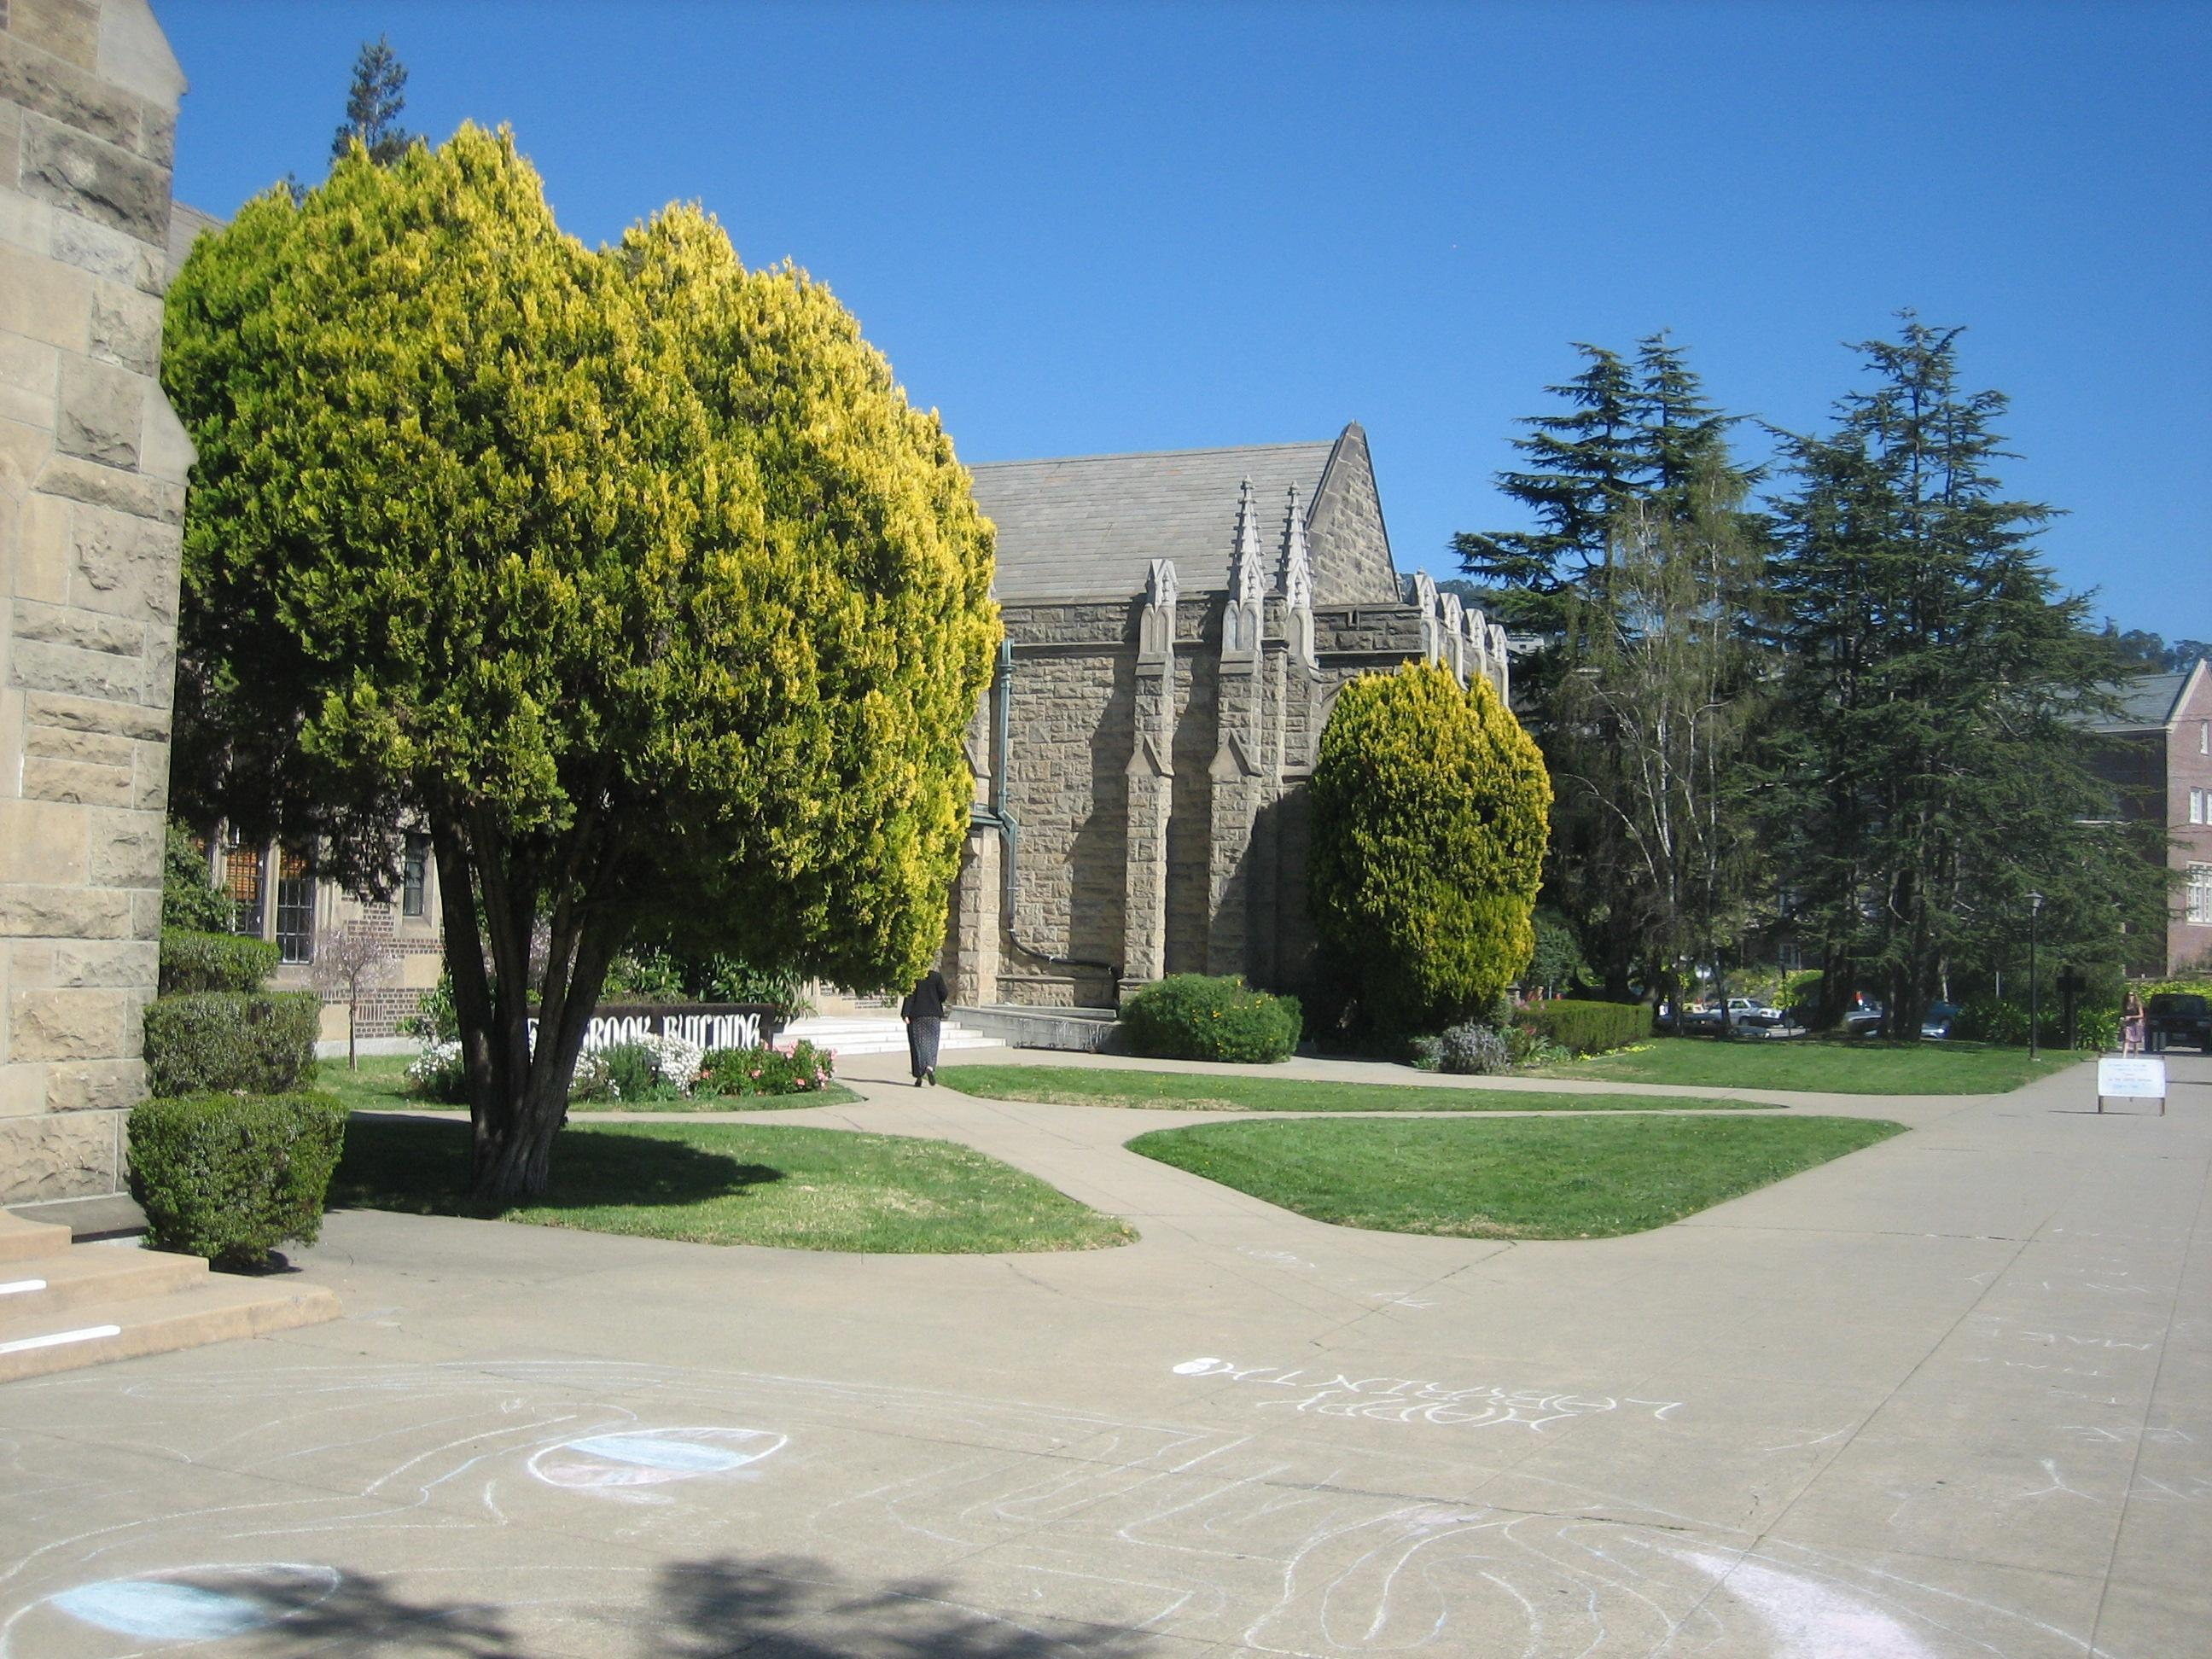
\includegraphics[width=10cm ,height=10cm ]{\input_image}};

        \pic[shift={(1, 0, 0)}, ] at (0,0,0)
            {RightBandedBox={
                name=conv_0_0,
                caption=,
                xlabel={(64,)},
                zlabel=I,
                fill=\ConvColor,
                bandfill=\ConvReluColor,
                height=40,
                depth=40,
                width={3.0}
                }
            };

        \draw [connection, ] (image_0) -- node  {\midarrow}(conv_0_0-west);

        \pic[shift={(2, 0, 0)}, ] at (conv_0_0-east)
            {RightBandedBox={
                name=conv_0_1,
                caption=,
                xlabel={(64,)},
                zlabel=I/2,
                fill=\ConvColor,
                bandfill=\ConvReluColor,
                height=20.0,
                depth=20.0,
                width={3.0}
                }
            };

        \draw [connection, ] (conv_0_0-east) -- node  {\midarrow}(conv_0_1-west);

        \draw[densely dashed]
            (conv_0_0-nearnortheast) coordinate(a) -- (conv_0_1-nearnorthwest)
            (conv_0_0-nearsoutheast) coordinate(b) -- (conv_0_1-nearsouthwest)
            (conv_0_0-farsoutheast) coordinate(c) -- (conv_0_1-farsouthwest)
            (conv_0_0-farnortheast) coordinate(d) -- (conv_0_1-farnorthwest)
            ;
    
        \pic[shift={(1, 0, 0)}, ] at (conv_0_1-east)
            {RightBandedBox={
                name=conv_1_0,
                caption=,
                xlabel={(64,)},
                zlabel=I/4,
                fill=\ConvColor,
                bandfill=\ConvReluColor,
                height=10.0,
                depth=10.0,
                width={3.0}
                }
            };

        \draw [connection, ] (conv_0_1-east) -- node  {\midarrow}(conv_1_0-west);

        \draw[densely dashed]
            (conv_0_1-nearnortheast) coordinate(a) -- (conv_1_0-nearnorthwest)
            (conv_0_1-nearsoutheast) coordinate(b) -- (conv_1_0-nearsouthwest)
            (conv_0_1-farsoutheast) coordinate(c) -- (conv_1_0-farsouthwest)
            (conv_0_1-farnortheast) coordinate(d) -- (conv_1_0-farnorthwest)
            ;
    
        \pic[shift={(1, 0, 0)}] at (conv_1_0-east)
            {Box={
                name=pool_0,
                caption= ,
                fill=\PoolColor,
                opacity=0.5,
                height=10.0,
                depth=10.0,
                width=2,
                }
            };

        \draw [connection, ] (conv_1_0-east) -- node  {\midarrow}(pool_0-west);

        \pic[shift={(1.5, 0, 0)}, ] at (pool_0-east)
            {RightBandedBox={
                name=bottleneck_1_0,
                caption=5,
                xlabel={(64,)},
                zlabel=,
                fill=\ConvColor,
                bandfill=\ConvReluColor,
                height=10.0,
                depth=10.0,
                width={3.0}
                }
            };

        \draw [connection, ] (pool_0-east) -- node [fillwhite](bottleneck_1_connection) {\midarrow}(bottleneck_1_0-west);

        \pic[shift={(0,0,0)}, ] at (bottleneck_1_0-east)
            {RightBandedBox={
                name=bottleneck_1_1,
                caption=6,
                xlabel={(64,)},
                zlabel=,
                fill=\ConvColor,
                bandfill=\ConvReluColor,
                height=10.0,
                depth=10.0,
                width={3.0}
                }
            };

        \pic[shift={(0,0,0)}, ] at (bottleneck_1_1-east)
            {RightBandedBox={
                name=bottleneck_1_2,
                caption=7,
                xlabel={(256,)},
                zlabel=,
                fill=\ConvColor,
                bandfill=\ConvReluColor,
                height=10.0,
                depth=10.0,
                width={4.0}
                }
            };

        \path (bottleneck_1_2-south) -- (bottleneck_1_2-north) coordinate[pos=1.5] (bottleneck_1_2-dummy) ;
        \path (bottleneck_1_2-dummy |- bottleneck_1_connection) coordinate (bottleneck_1_connection-dummy)  ;

        \draw [connection] 
            (bottleneck_1_connection)
            -- node {}(bottleneck_1_connection |- bottleneck_1_2-dummy)
            -- node {\midarrow}(bottleneck_1_2-dummy -| bottleneck_1_2-south)
            -- node {}(bottleneck_1_2-north)
;
    
        \pic[shift={(1.5, 0, 0)}, ] at (bottleneck_1_2-east)
            {RightBandedBox={
                name=bottleneck_2_0,
                caption=8,
                xlabel={(64,)},
                zlabel=,
                fill=\ConvColor,
                bandfill=\ConvReluColor,
                height=10.0,
                depth=10.0,
                width={3.0}
                }
            };

        \draw [connection, ] (bottleneck_1_2-east) -- node [fillwhite](bottleneck_2_connection) {\midarrow}(bottleneck_2_0-west);

        \pic[shift={(0,0,0)}, ] at (bottleneck_2_0-east)
            {RightBandedBox={
                name=bottleneck_2_1,
                caption=9,
                xlabel={(64,)},
                zlabel=,
                fill=\ConvColor,
                bandfill=\ConvReluColor,
                height=10.0,
                depth=10.0,
                width={3.0}
                }
            };

        \pic[shift={(0,0,0)}, ] at (bottleneck_2_1-east)
            {RightBandedBox={
                name=bottleneck_2_2,
                caption=10,
                xlabel={(256,)},
                zlabel=,
                fill=\ConvColor,
                bandfill=\ConvReluColor,
                height=10.0,
                depth=10.0,
                width={4.0}
                }
            };

        \path (bottleneck_2_2-south) -- (bottleneck_2_2-north) coordinate[pos=1.5] (bottleneck_2_2-dummy) ;
        \path (bottleneck_2_2-dummy |- bottleneck_2_connection) coordinate (bottleneck_2_connection-dummy)  ;

        \draw [connection] 
            (bottleneck_2_connection)
            -- node {}(bottleneck_2_connection |- bottleneck_2_2-dummy)
            -- node {\midarrow}(bottleneck_2_2-dummy -| bottleneck_2_2-south)
            -- node {}(bottleneck_2_2-north)
;
    
        \pic[shift={(1.5, 0, 0)}, ] at (bottleneck_2_2-east)
            {RightBandedBox={
                name=bottleneck_3_0,
                caption=11,
                xlabel={(64,)},
                zlabel=,
                fill=\ConvColor,
                bandfill=\ConvReluColor,
                height=10.0,
                depth=10.0,
                width={3.0}
                }
            };

        \draw [connection, ] (bottleneck_2_2-east) -- node [fillwhite](bottleneck_3_connection) {\midarrow}(bottleneck_3_0-west);

        \pic[shift={(0,0,0)}, ] at (bottleneck_3_0-east)
            {RightBandedBox={
                name=bottleneck_3_1,
                caption=12,
                xlabel={(64,)},
                zlabel=,
                fill=\ConvColor,
                bandfill=\ConvReluColor,
                height=10.0,
                depth=10.0,
                width={3.0}
                }
            };

        \pic[shift={(0,0,0)}, ] at (bottleneck_3_1-east)
            {RightBandedBox={
                name=bottleneck_3_2,
                caption=13,
                xlabel={(256,)},
                zlabel=,
                fill=\ConvColor,
                bandfill=\ConvReluColor,
                height=10.0,
                depth=10.0,
                width={4.0}
                }
            };

        \path (bottleneck_3_2-south) -- (bottleneck_3_2-north) coordinate[pos=1.5] (bottleneck_3_2-dummy) ;
        \path (bottleneck_3_2-dummy |- bottleneck_3_connection) coordinate (bottleneck_3_connection-dummy)  ;

        \draw [connection] 
            (bottleneck_3_connection)
            -- node {}(bottleneck_3_connection |- bottleneck_3_2-dummy)
            -- node {\midarrow}(bottleneck_3_2-dummy -| bottleneck_3_2-south)
            -- node {}(bottleneck_3_2-north)
;
    
        \pic[shift={(3, 0, 0)}, ] at (bottleneck_3_2-east)
            {RightBandedBox={
                name=bottleneck_4_0,
                caption=14,
                xlabel={(128,)},
                zlabel=,
                fill=\ConvColor,
                bandfill=\ConvReluColor,
                height=5.0,
                depth=5.0,
                width={3.5}
                }
            };

        \draw [connection, ] (bottleneck_3_2-east) -- node [fillwhite](bottleneck_4_connection) {\midarrow}(bottleneck_4_0-west);

        \pic[shift={(0,0,0)}, ] at (bottleneck_4_0-east)
            {RightBandedBox={
                name=bottleneck_4_1,
                caption=15,
                xlabel={(128,)},
                zlabel=,
                fill=\ConvColor,
                bandfill=\ConvReluColor,
                height=5.0,
                depth=5.0,
                width={3.5}
                }
            };

        \pic[shift={(0,0,0)}, ] at (bottleneck_4_1-east)
            {RightBandedBox={
                name=bottleneck_4_2,
                caption=16,
                xlabel={(512,)},
                zlabel=,
                fill=\ConvColor,
                bandfill=\ConvReluColor,
                height=5.0,
                depth=5.0,
                width={4.5}
                }
            };

        \path (bottleneck_4_2-south) -- (bottleneck_4_2-north) coordinate[pos=1.5] (bottleneck_4_2-dummy) ;
        \path (bottleneck_4_2-dummy |- bottleneck_4_connection) coordinate (bottleneck_4_connection-dummy)  ;

        \draw [connection] 
            (bottleneck_4_connection)
            -- node {}(bottleneck_4_connection |- bottleneck_4_2-dummy)
            -- node {\midarrow}(bottleneck_4_2-dummy -| bottleneck_4_2-south)
            -- node {}(bottleneck_4_2-north)
;
    
        \pic[shift={(1.5, 0, 0)}, ] at (bottleneck_4_2-east)
            {RightBandedBox={
                name=bottleneck_7_0,
                caption=24,
                xlabel={(128,)},
                zlabel=,
                fill=\ConvColor,
                bandfill=\ConvReluColor,
                height=5.0,
                depth=5.0,
                width={3.5}
                }
            };

        \draw [connection] (bottleneck_4_2-east) -- node [fill=white,inner sep=1pt, opacity=1]{\ldots} (bottleneck_7_0-west);
    
        \coordinate [shift={(-0.25,0,0)}] (bottleneck_7_connection) at (bottleneck_7_0-west);
        
        \pic[shift={(0,0,0)}, ] at (bottleneck_7_0-east)
            {RightBandedBox={
                name=bottleneck_7_1,
                caption=25,
                xlabel={(128,)},
                zlabel=,
                fill=\ConvColor,
                bandfill=\ConvReluColor,
                height=5.0,
                depth=5.0,
                width={3.5}
                }
            };

        \pic[shift={(0,0,0)}, ] at (bottleneck_7_1-east)
            {RightBandedBox={
                name=bottleneck_7_2,
                caption=26,
                xlabel={(512,)},
                zlabel=,
                fill=\ConvColor,
                bandfill=\ConvReluColor,
                height=5.0,
                depth=5.0,
                width={4.5}
                }
            };

        \path (bottleneck_7_2-south) -- (bottleneck_7_2-north) coordinate[pos=1.5] (bottleneck_7_2-dummy) ;
        \path (bottleneck_7_2-dummy |- bottleneck_7_connection) coordinate (bottleneck_7_connection-dummy)  ;

        \draw [connection] 
            (bottleneck_7_connection)
            -- node {}(bottleneck_7_connection |- bottleneck_7_2-dummy)
            -- node {\midarrow}(bottleneck_7_2-dummy -| bottleneck_7_2-south)
            -- node {}(bottleneck_7_2-north)
;
    
        \pic[shift={(1.5, 0, 0)}, ] at (bottleneck_7_2-east)
            {RightBandedBox={
                name=bottleneck_8_0,
                caption=27,
                xlabel={(256,)},
                zlabel=,
                fill=\ConvColor,
                bandfill=\ConvReluColor,
                height=2.5,
                depth=2.5,
                width={4.0}
                }
            };

        \draw [connection, ] (bottleneck_7_2-east) -- node [fillwhite](bottleneck_8_connection) {\midarrow}(bottleneck_8_0-west);

        \pic[shift={(0,0,0)}, ] at (bottleneck_8_0-east)
            {RightBandedBox={
                name=bottleneck_8_1,
                caption=28,
                xlabel={(256,)},
                zlabel=,
                fill=\ConvColor,
                bandfill=\ConvReluColor,
                height=2.5,
                depth=2.5,
                width={4.0}
                }
            };

        \pic[shift={(0,0,0)}, ] at (bottleneck_8_1-east)
            {RightBandedBox={
                name=bottleneck_8_2,
                caption=29,
                xlabel={(1024,)},
                zlabel=,
                fill=\ConvColor,
                bandfill=\ConvReluColor,
                height=2.5,
                depth=2.5,
                width={5.0}
                }
            };

        \path (bottleneck_8_2-south) -- (bottleneck_8_2-north) coordinate[pos=2] (bottleneck_8_2-dummy) ;
        \path (bottleneck_8_2-dummy |- bottleneck_8_connection) coordinate (bottleneck_8_connection-dummy)  ;

        \draw [connection] 
            (bottleneck_8_connection)
            -- node {}(bottleneck_8_connection |- bottleneck_8_2-dummy)
            -- node {\midarrow}(bottleneck_8_2-dummy -| bottleneck_8_2-south)
            -- node {}(bottleneck_8_2-north)
;
    
        \pic[shift={(1.5, 0, 0)}, ] at (bottleneck_8_2-east)
            {RightBandedBox={
                name=bottleneck_13_0,
                caption=43,
                xlabel={(256,)},
                zlabel=,
                fill=\ConvColor,
                bandfill=\ConvReluColor,
                height=2.5,
                depth=2.5,
                width={4.0}
                }
            };

        \draw [connection] (bottleneck_8_2-east) -- node [fill=white,inner sep=1pt, opacity=1]{\ldots} (bottleneck_13_0-west);
    
        \coordinate [shift={(-0.25,0,0)}] (bottleneck_13_connection) at (bottleneck_13_0-west);
        
        \pic[shift={(0,0,0)}, ] at (bottleneck_13_0-east)
            {RightBandedBox={
                name=bottleneck_13_1,
                caption=44,
                xlabel={(256,)},
                zlabel=,
                fill=\ConvColor,
                bandfill=\ConvReluColor,
                height=2.5,
                depth=2.5,
                width={4.0}
                }
            };

        \pic[shift={(0,0,0)}, ] at (bottleneck_13_1-east)
            {RightBandedBox={
                name=bottleneck_13_2,
                caption=45,
                xlabel={(1024,)},
                zlabel=,
                fill=\ConvColor,
                bandfill=\ConvReluColor,
                height=2.5,
                depth=2.5,
                width={5.0}
                }
            };

        \path (bottleneck_13_2-south) -- (bottleneck_13_2-north) coordinate[pos=2] (bottleneck_13_2-dummy) ;
        \path (bottleneck_13_2-dummy |- bottleneck_13_connection) coordinate (bottleneck_13_connection-dummy)  ;

        \draw [connection] 
            (bottleneck_13_connection)
            -- node {}(bottleneck_13_connection |- bottleneck_13_2-dummy)
            -- node {\midarrow}(bottleneck_13_2-dummy -| bottleneck_13_2-south)
            -- node {}(bottleneck_13_2-north)
;
    
        \pic[shift={(1.5, 0, 0)}, ] at (bottleneck_13_2-east)
            {RightBandedBox={
                name=bottleneck_14_0,
                caption=46,
                xlabel={(512,)},
                zlabel=,
                fill=\ConvColor,
                bandfill=\ConvReluColor,
                height=1.25,
                depth=1.25,
                width={4.5}
                }
            };

        \draw [connection, ] (bottleneck_13_2-east) -- node [fillwhite](bottleneck_14_connection) {\midarrow}(bottleneck_14_0-west);

        \pic[shift={(0,0,0)}, ] at (bottleneck_14_0-east)
            {RightBandedBox={
                name=bottleneck_14_1,
                caption=47,
                xlabel={(512,)},
                zlabel=,
                fill=\ConvColor,
                bandfill=\ConvReluColor,
                height=1.25,
                depth=1.25,
                width={4.5}
                }
            };

        \pic[shift={(0,0,0)}, ] at (bottleneck_14_1-east)
            {RightBandedBox={
                name=bottleneck_14_2,
                caption=48,
                xlabel={(2048,)},
                zlabel=,
                fill=\ConvColor,
                bandfill=\ConvReluColor,
                height=1.25,
                depth=1.25,
                width={5.5}
                }
            };

        \path (bottleneck_14_2-south) -- (bottleneck_14_2-north) coordinate[pos=3] (bottleneck_14_2-dummy) ;
        \path (bottleneck_14_2-dummy |- bottleneck_14_connection) coordinate (bottleneck_14_connection-dummy)  ;

        \draw [connection] 
            (bottleneck_14_connection)
            -- node {}(bottleneck_14_connection |- bottleneck_14_2-dummy)
            -- node {\midarrow}(bottleneck_14_2-dummy -| bottleneck_14_2-south)
            -- node {}(bottleneck_14_2-north)
;
    
        \pic[shift={(1.5, 0, 0)}, ] at (bottleneck_14_2-east)
            {RightBandedBox={
                name=bottleneck_16_0,
                caption=53,
                xlabel={(512,)},
                zlabel=,
                fill=\ConvColor,
                bandfill=\ConvReluColor,
                height=1.25,
                depth=1.25,
                width={4.5}
                }
            };

        \draw [connection] (bottleneck_14_2-east) -- node [fill=white,inner sep=1pt, opacity=1]{\ldots} (bottleneck_16_0-west);
    
        \coordinate [shift={(-0.25,0,0)}] (bottleneck_16_connection) at (bottleneck_16_0-west);
        
        \pic[shift={(0,0,0)}, ] at (bottleneck_16_0-east)
            {RightBandedBox={
                name=bottleneck_16_1,
                caption=54,
                xlabel={(512,)},
                zlabel=,
                fill=\ConvColor,
                bandfill=\ConvReluColor,
                height=1.25,
                depth=1.25,
                width={4.5}
                }
            };

        \pic[shift={(0,0,0)}, ] at (bottleneck_16_1-east)
            {RightBandedBox={
                name=bottleneck_16_2,
                caption=55,
                xlabel={(2048,)},
                zlabel=,
                fill=\ConvColor,
                bandfill=\ConvReluColor,
                height=1.25,
                depth=1.25,
                width={5.5}
                }
            };

        \path (bottleneck_16_2-south) -- (bottleneck_16_2-north) coordinate[pos=3] (bottleneck_16_2-dummy) ;
        \path (bottleneck_16_2-dummy |- bottleneck_16_connection) coordinate (bottleneck_16_connection-dummy)  ;

        \draw [connection] 
            (bottleneck_16_connection)
            -- node {}(bottleneck_16_connection |- bottleneck_16_2-dummy)
            -- node {\midarrow}(bottleneck_16_2-dummy -| bottleneck_16_2-south)
            -- node {}(bottleneck_16_2-north)
;
    
    	\coordinate [shift={(3, 0, 0)}] (resnet_last_dummy) at (bottleneck_16_2-east);
    
    	\coordinate [shift={(0, 0, 6)}] (resnet_connection_dummy) at (resnet_last_dummy);
    
        \draw [connection, ] (bottleneck_16_2-east) -- node [fillwhite] {\midarrow}(resnet_last_dummy);

        \draw [connection, ] (resnet_last_dummy) -- node [fillwhite] {\midarrow}(resnet_connection_dummy);

        \pic[shift={(0, -5, 0)}] at (bottleneck_16_2-center)
            {Box={
                name=pool_1,
                caption= ,
                fill=\PoolColor,
                opacity=0.5,
                height=10.0,
                depth=10.0,
                width=2,
                }
            };

        \pic[shift={(-2.5, 0, 0)}, ] at (pool_1-west)
            {LeftBandedBox={
                name=conv_pool_1,
                caption=,
                xlabel={(512,)},
                zlabel=,
                fill=\ConvColor,
                bandfill=\ConvReluColor,
                height=1.25,
                depth=1.25,
                width={4.5}
                }
            };

        \draw [connection, pos=0.75] (pool_1-west) -- node [fillwhite] {\midarrow}(conv_pool_1-east);

        \pic[shift={(0, 0, 5)}] at (pool_1-center)
            {Box={
                name=pool_2,
                caption= ,
                fill=\PoolColor,
                opacity=0.5,
                height=10.0,
                depth=10.0,
                width=2,
                }
            };

	\node[canvas is zy plane at x=0](grid_2) at (pool_2-east) {\drawcoloredgrid{2}{2}{1.0}{black}};

        \pic[shift={(-2.5, 0, 0)}, ] at (pool_2-west)
            {LeftBandedBox={
                name=conv_pool_2,
                caption=,
                xlabel={(512,)},
                zlabel=,
                fill=\ConvColor,
                bandfill=\ConvReluColor,
                height=1.25,
                depth=1.25,
                width={4.5}
                }
            };

        \draw [connection, pos=0.75] (pool_2-west) -- node [fillwhite] {\midarrow}(conv_pool_2-east);

        \pic[shift={(0, 0, 5)}] at (pool_2-center)
            {Box={
                name=pool_3,
                caption= ,
                fill=\PoolColor,
                opacity=0.5,
                height=10.0,
                depth=10.0,
                width=2,
                }
            };

	\node[canvas is zy plane at x=0](grid_3) at (pool_3-east) {\drawcoloredgrid{2}{2}{0.5}{black}};

        \pic[shift={(-2.5, 0, 0)}, ] at (pool_3-west)
            {LeftBandedBox={
                name=conv_pool_3,
                caption=,
                xlabel={(512,)},
                zlabel=,
                fill=\ConvColor,
                bandfill=\ConvReluColor,
                height=1.25,
                depth=1.25,
                width={4.5}
                }
            };

        \draw [connection, pos=0.75] (pool_3-west) -- node [fillwhite] {\midarrow}(conv_pool_3-east);

        \pic[shift={(0, 0, 5)}] at (pool_3-center)
            {Box={
                name=pool_4,
                caption= ,
                fill=\PoolColor,
                opacity=0.5,
                height=10.0,
                depth=10.0,
                width=2,
                }
            };

	\node[canvas is zy plane at x=0](grid_4) at (pool_4-east) {\drawcoloredgrid{2}{2}{0.25}{black}};

        \pic[shift={(-2.5, 0, 0)}, ] at (pool_4-west)
            {LeftBandedBox={
                name=conv_pool_4,
                caption=,
                xlabel={(512,)},
                zlabel=,
                fill=\ConvColor,
                bandfill=\ConvReluColor,
                height=1.25,
                depth=1.25,
                width={4.5}
                }
            };

        \draw [connection, pos=0.75] (pool_4-west) -- node [fillwhite] {\midarrow}(conv_pool_4-east);

        \pic[shift={(-5, 0, 2.5)}] at (pool_2-east)
            {Ball={
                name=conc_1,
                caption=,
                fill=\ConcColor,
                opacity=0.6,
                radius=2.5,
                logo=$\oplus$
                }
            };
    
    	\coordinate [shift={(5, 0, 0)}] (dummy_pool_1) at (pool_1-east);
    
    	\coordinate [shift={(5, 0, 0)}] (dummy_pool_2) at (pool_2-east);
    
    	\coordinate [shift={(5, 0, 0)}] (dummy_pool_3) at (pool_3-east);
    
    	\coordinate [shift={(5, 0, 0)}] (dummy_pool_4) at (pool_4-east);
    
        \draw [connection, ] (dummy_pool_1) -- node [fillwhite] {\midarrow}(pool_1-east);

        \draw [connection, ] (dummy_pool_1) -- node {} (dummy_pool_2) -- node [fillwhite] {\midarrow}(pool_2-east);

        \draw [connection, ] (dummy_pool_2) -- node {} (dummy_pool_3) -- node [fillwhite] {\midarrow}(pool_3-east);

        \draw [connection, ] (dummy_pool_3) -- node {} (dummy_pool_4) -- node [fillwhite] {\midarrow}(pool_4-east);

        \draw [connection]  (resnet_last_dummy)    -- node {} ++(6, 0, 0) -- node {\midarrow} (dummy_pool_1);
    
        \draw [connection]  (conv_pool_1-west)    -- node {} ++(-2, 0, 0) -- node {\midarrow} (conc_1-northeast);
    
        \draw [connection]  (conv_pool_2-west)    -- node {} ++(0, 0, 0) -- node {\midarrow} (conc_1-east);
    
        \draw [connection]  (conv_pool_3-west)    -- node {} ++(0, 0, 0) -- node {\midarrow} (conc_1-southeast);
    
        \draw [connection]  (conv_pool_4-west)    -- node {} ++(-2, 0, 0) -- node {\midarrow} (conc_1-southwest);
    
        \draw [connection]  (resnet_connection_dummy)    -- node {} ++(-4.5, 0, 0) -- node {\midarrow} (conc_1-northwest);
    
        \pic[shift={(-2.5, 0, 0)}, ] at (conc_1-west)
            {RightBandedBox={
                name=conv_60,
                caption=60,
                xlabel={(512,)},
                zlabel=,
                fill=\ConvColor,
                bandfill=\ConvReluColor,
                height=1.25,
                depth=1.25,
                width={4.5}
                }
            };

        \draw [connection, pos=0.75] (conc_1-west) -- node [fillwhite] {\midarrow}(conv_60-east);

        \pic[shift={(-2.5, 0, 0)}, ] at (conc_1-west)
            {LeftBandedBox={
                name=conv_60,
                caption=,
                xlabel={(512,)},
                zlabel=,
                fill=\ConvColor,
                bandfill=\ConvReluColor,
                height=1.25,
                depth=1.25,
                width={4.5}
                }
            };

        \pic[shift={(0.4, 0, 8)}, rotate = -100] at (bottleneck_14_connection)
            {RightBandedBox={
                name=conv_61,
                caption= ,
                xlabel={(512,)},
                zlabel=,
                fill=\ConvColor,
                bandfill=\ConvReluColor,
                height=2.5,
                depth=2.5,
                width={2}
                }
            };

        \draw [connection, ] (bottleneck_14_connection) -- node [fillwhite] {\midarrow}(conv_61-west);

        \pic[shift={(-3, 2, 0)}] at (conv_60-east)
            {Ball={
                name=sum_1,
                caption=,
                fill=\SumColor,
                opacity=0.4,
                radius=2.5,
                logo=$+$
                }
            };
    
        \draw [connection, ] (conv_61-east) -- node [fillwhite] {\midarrow}(sum_1-northeast);

        \pic[shift={(-2.5, 0, 0)}] at (sum_1-west)
            {Box={
                name=up_1_0,
                fill=\UpsampleColor,
                height=2.5,
                depth=2.5,
                width={1}
                }
            };
        \pic[shift={(-2.5, 0, 0)}] at (up_1_0-east)
            {Box={
                name=up_1,
                fill=\UpsampleColor,
                height=5.0,
                depth=5.0,
                width={1}
                }
            };
        \draw[densely dashed]
            (up_1_0-nearnortheast) coordinate(a) -- (up_1-nearnorthwest)
            (up_1_0-nearsoutheast) coordinate(b) -- (up_1-nearsouthwest)
            (up_1_0-farsoutheast) coordinate(c) -- (up_1-farsouthwest)
            (up_1_0-farnortheast) coordinate(d) -- (up_1-farnorthwest)

            (a)--(b)--(c)--(d)
            ;

        \draw [connection, ] (sum_1-west) -- node [fillwhite] {\midarrow}(up_1_0-west);

        \pic[shift={(-5.5, 0, 9.4)}, ] at (conv_60-west)
            {LeftBandedBox={
                name=conv_62,
                caption=62,
                xlabel={(512,)},
                zlabel=,
                fill=\ConvColor,
                bandfill=\ConvReluColor,
                height=2.5,
                depth=2.5,
                width={4.5}
                }
            };

        \draw [connection]  (conv_60-farwest)    -- node {} ++(-0.3, 0, -5) -- node {\midarrow} (sum_1-east);
    
        \pic[shift={(0.5, 0, 8)}, rotate = -100] at (bottleneck_8_connection)
            {RightBandedBox={
                name=conv_63,
                caption= ,
                xlabel={(512,)},
                zlabel=,
                fill=\ConvColor,
                bandfill=\ConvReluColor,
                height=5.0,
                depth=5.0,
                width={2}
                }
            };

        \draw [connection, ] (bottleneck_8_connection) -- node [fillwhite] {\midarrow}(conv_63-west);

        \pic[shift={(-3, 0, 0)}] at (up_1-east)
            {Ball={
                name=sum_2,
                caption=,
                fill=\SumColor,
                opacity=0.4,
                radius=2.5,
                logo=$+$
                }
            };
    
        \draw [connection, ] (conv_63-east) -- node [fillwhite] {\midarrow}(sum_2-northeast);

        \draw [connection, ] (up_1-west) -- node [fillwhite] {\midarrow}(sum_2-east);

        \pic[shift={(-2.5, 0, 0)}] at (sum_2-west)
            {Box={
                name=up_2_0,
                fill=\UpsampleColor,
                height=5.0,
                depth=5.0,
                width={1}
                }
            };
        \pic[shift={(-2.5, 0, 0)}] at (up_2_0-east)
            {Box={
                name=up_2,
                fill=\UpsampleColor,
                height=10.0,
                depth=10.0,
                width={1}
                }
            };
        \draw[densely dashed]
            (up_2_0-nearnortheast) coordinate(a) -- (up_2-nearnorthwest)
            (up_2_0-nearsoutheast) coordinate(b) -- (up_2-nearsouthwest)
            (up_2_0-farsoutheast) coordinate(c) -- (up_2-farsouthwest)
            (up_2_0-farnortheast) coordinate(d) -- (up_2-farnorthwest)

            (a)--(b)--(c)--(d)
            ;

        \draw [connection, ] (sum_2-west) -- node [fillwhite] {\midarrow}(up_2_0-west);

        \pic[shift={(0.2, 0, 5)}, rotate=-100] at (up_1-south)
            {RightBandedBox={
                name=conv_64,
                caption= ,
                xlabel={(512,)},
                zlabel=,
                fill=\ConvColor,
                bandfill=\ConvReluColor,
                height=5.0,
                depth=5.0,
                width={2}
                }
            };

        \draw [connection, ] (up_1-nearsouthwest) -- node [fillwhite] {\midarrow}(conv_64-west);

        \pic[shift={(0.6, 0, 9)}, rotate = -100] at (bottleneck_4_connection)
            {RightBandedBox={
                name=conv_65,
                caption= ,
                xlabel={(512,)},
                zlabel=,
                fill=\ConvColor,
                bandfill=\ConvReluColor,
                height=10.0,
                depth=10.0,
                width={2}
                }
            };

        \draw [connection, ] (bottleneck_4_connection) -- node [fillwhite] {\midarrow}(conv_65-west);

        \pic[shift={(-3, 0, 0)}] at (up_2-east)
            {Ball={
                name=sum_3,
                caption=,
                fill=\SumColor,
                opacity=0.4,
                radius=2.5,
                logo=$+$
                }
            };
    
        \draw [connection, ] (conv_65-east) -- node [fillwhite] {\midarrow}(sum_3-northeast);

        \draw [connection, ] (up_2-west) -- node [fillwhite] {\midarrow}(sum_3-east);

        \pic[shift={(0.2, 0, 4)}, rotate=-100] at (up_2-south)
            {RightBandedBox={
                name=conv_66,
                caption= ,
                xlabel={(512,)},
                zlabel=,
                fill=\ConvColor,
                bandfill=\ConvReluColor,
                height=10.0,
                depth=10.0,
                width={2}
                }
            };

        \draw [connection, ] (up_2-nearsouthwest) -- node [fillwhite] {\midarrow}(conv_66-west);

        \pic[shift={(-2.5, 0, 0)}, ] at (sum_3-west)
            {LeftBandedBox={
                name=up_3,
                caption=,
                xlabel={(512,)},
                zlabel=,
                fill=\ConvColor,
                bandfill=\ConvReluColor,
                height=10.0,
                depth=10.0,
                width={4.5}
                }
            };

        \draw [connection, ] (sum_3-west) -- node [fillwhite] {\midarrow}(up_3-east);

        \pic[shift={(0, -5, 0)}] at (sum_3-east)
            {Ball={
                name=conc_2,
                caption=,
                fill=\ConcColor,
                opacity=0.6,
                radius=2.5,
                logo=$\oplus$
                }
            };
    
        \draw [connection]  (conv_60-nearwest)    -- node {} ++(-1, -2, 4) -- node {\midarrow} (conv_62-east);
    
        \draw [connection]  (conv_64-east)    -- node {} ++(-1, -1.5, 2) -- node {\midarrow} (conc_2-east);
    
        \draw [connection, ] (conv_62-east) -- node [fillwhite] {\midarrow}(conc_2-south);

        \draw [connection]  (conv_66-east)    -- node {} ++(0, 0, 0) -- node {\midarrow} (conc_2-north);
    
        \draw [connection]  (up_3-nearsouthwest)    -- node {} ++(0, 0, 9) -- node {\midarrow} (conc_2-west);
    
        \pic[shift={(-4, 0, 8)}, ] at (conc_2-east)
            {LeftBandedBox={
                name=conv_67,
                caption=,
                xlabel={(512,)},
                zlabel=,
                fill=\ConvColor,
                bandfill=\ConvReluColor,
                height=10.0,
                depth=10.0,
                width={4.5}
                }
            };

        \draw [connection]  (conc_2-southwest)    -- node {} ++(0, 0, 7.1) -- node {\midarrow} (conv_67-east);
    
        \pic[shift={(-3.5, 0, 0)}, ] at (conv_67-west)
            {LeftBandedBox={
                name=conv_68,
                caption=,
                xlabel={(128,)},
                zlabel=,
                fill=\ConvColor,
                bandfill=\ConvReluColor,
                height=10.0,
                depth=10.0,
                width={3.5}
                }
            };

        \draw [connection, ] (conv_67-west) -- node [fillwhite] {\midarrow}(conv_68-east);

        \pic[shift={(-2, 0, 0)}] at (conv_68-west)
            {Box={
                name=soft_max,
                caption= ,
                xlabel={{32,}},
                zlabel=,
                fill=\SoftmaxColor,
                opacity=0.8,
                height=10.0,
                depth=10.0,
                width=1.5
                }
            };

        \draw [connection, ] (conv_68-west) -- node [fillwhite] {\midarrow}(soft_max-east);

    \pic[shift={(-2, 0, 0)}] at (soft_max-west)
		{Box={
            name=image_1,
            caption= ,
            zlabel=,
            fill=white,
            opacity=0.8,
            height=10.0,
            depth=10.0,
            width=0.5
        }
    };

    \pic[shift={(-4, 0, 0)}] at (image_1-west)
    {Box={
        name=image_2,
        caption= ,
        zlabel=,
        fill=white,
        opacity=0.8,
        height=40.0,
        depth=40.0,
        width=0.5
        }
    };

    \node[canvas is zy plane at x=0] (img_1) at (image_1-east) {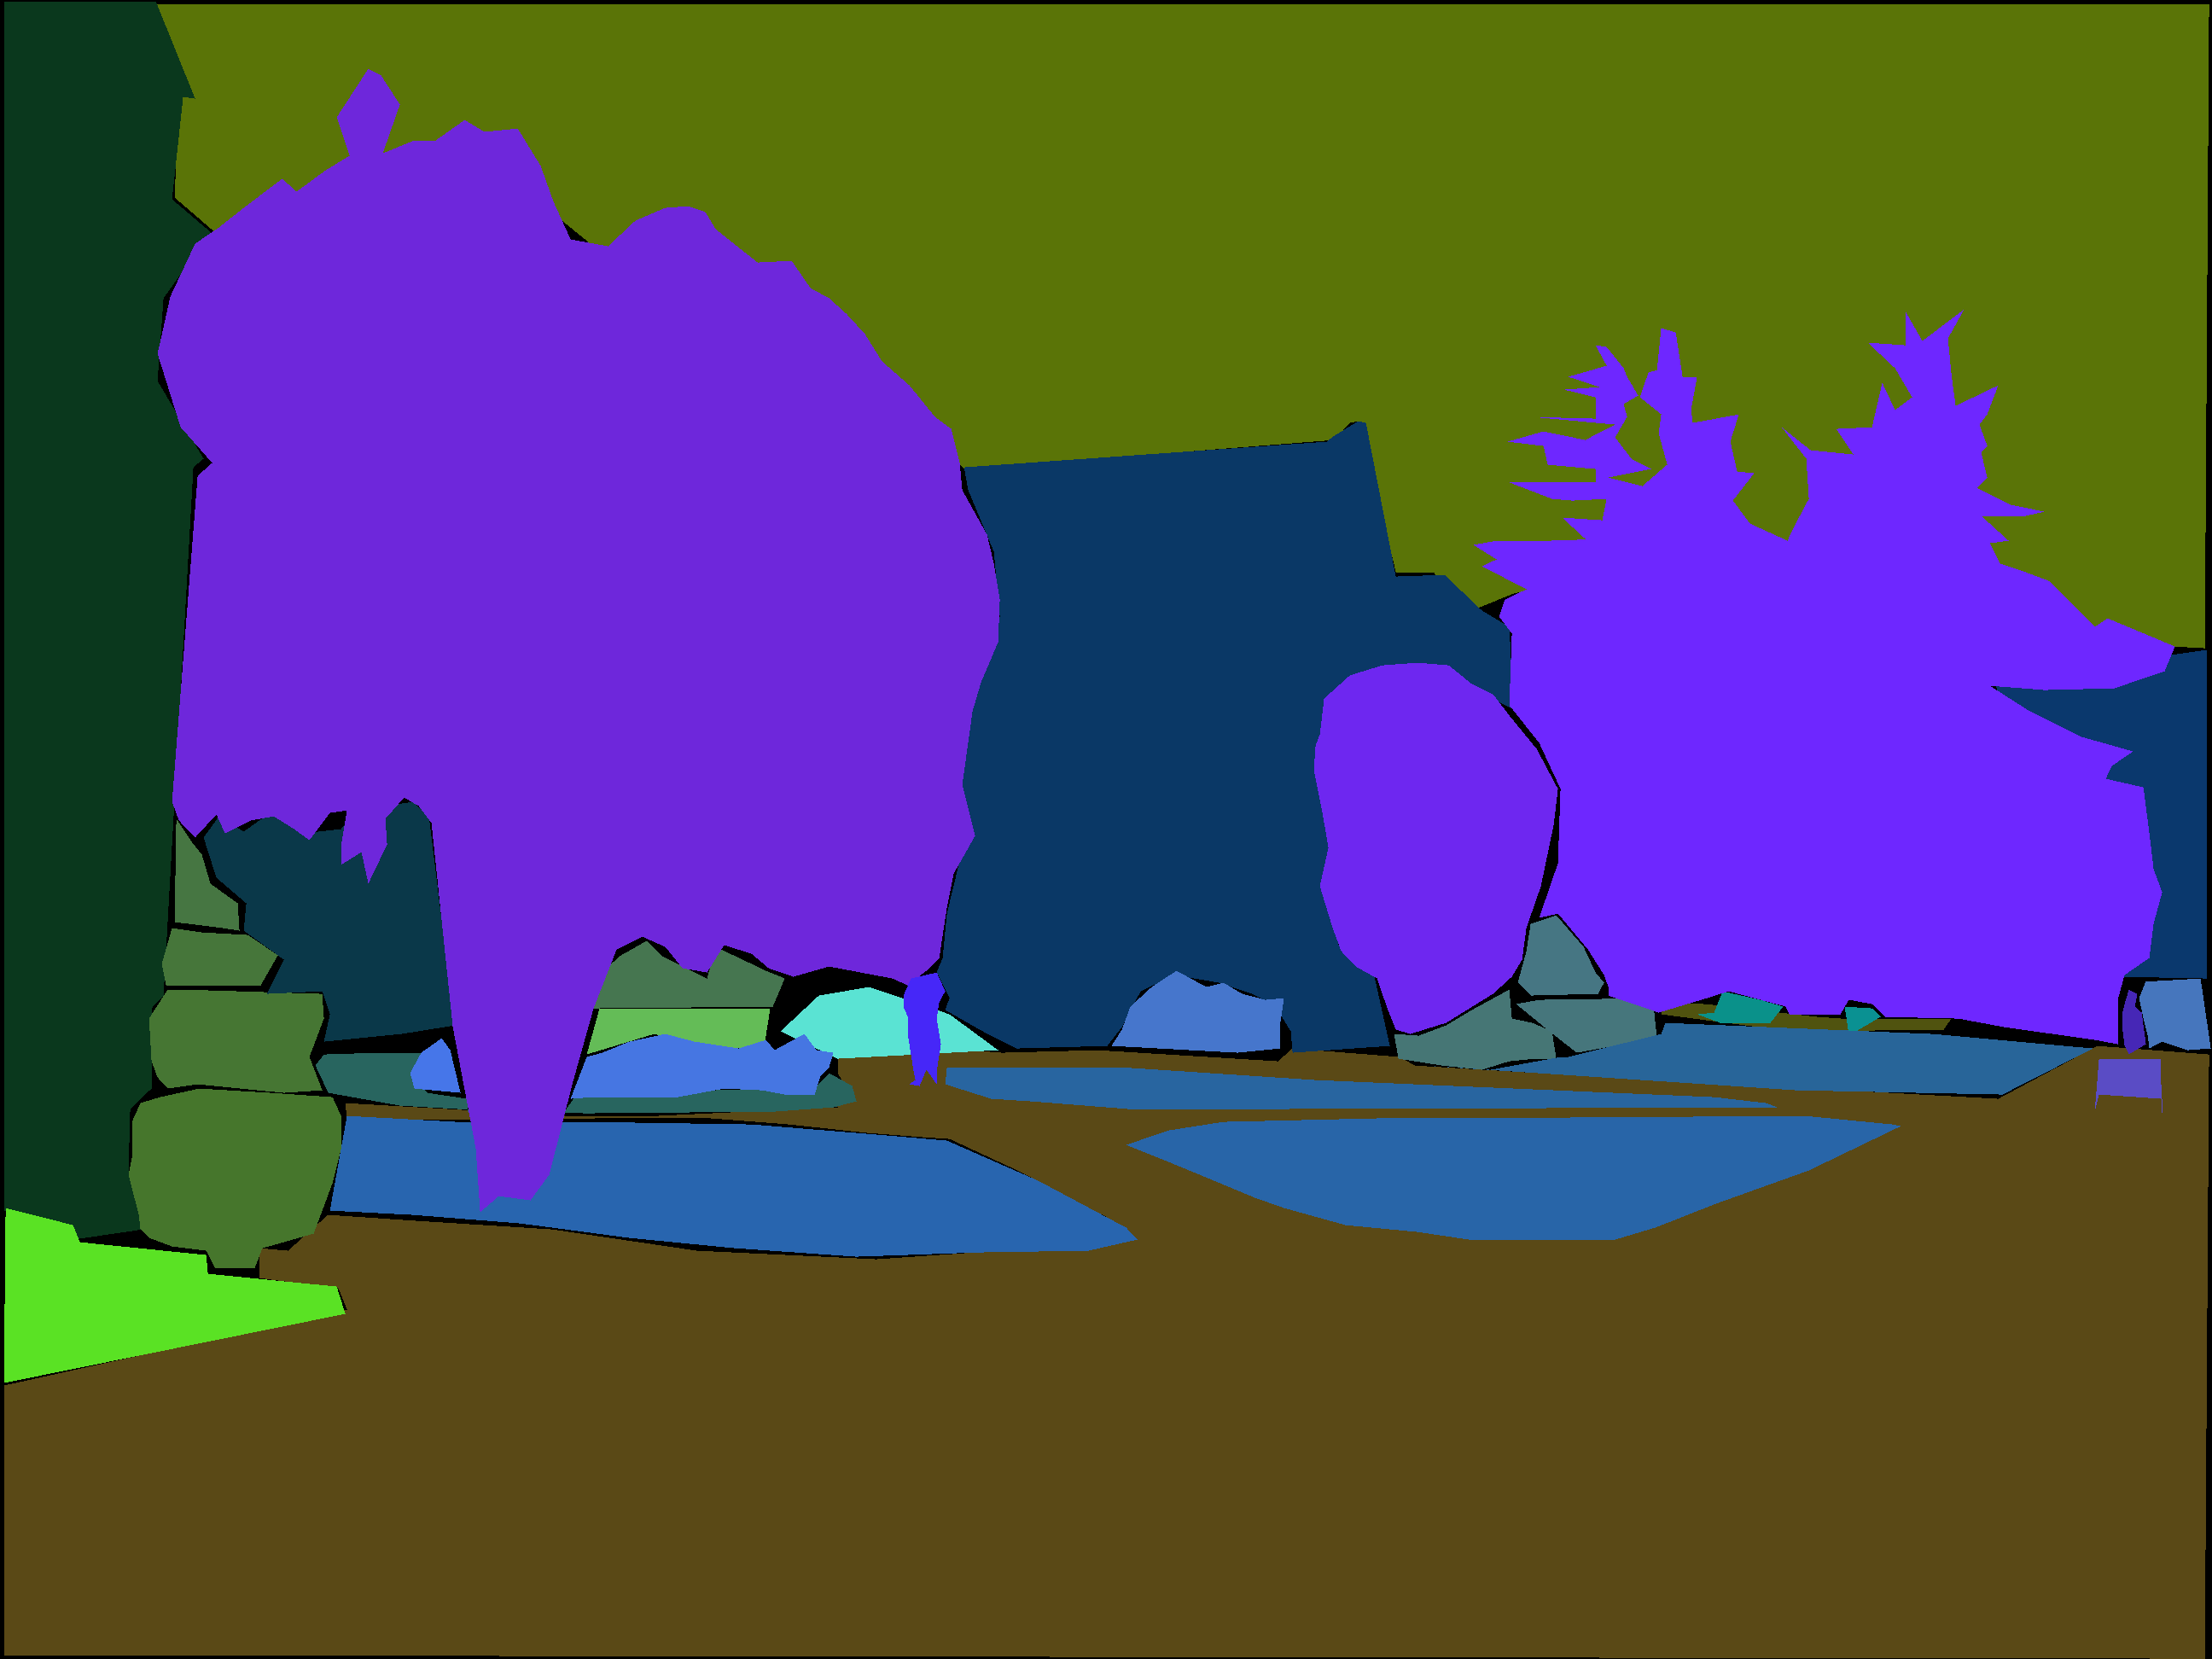
\includegraphics[width=2cm,height=2cm]{\output_image}};

    \draw [connection] (soft_max-east) -- node [fillwhite] {\midarrow}(image_1-west);

    \node[canvas is zy plane at x=0] (img_2) at (image_2-east) {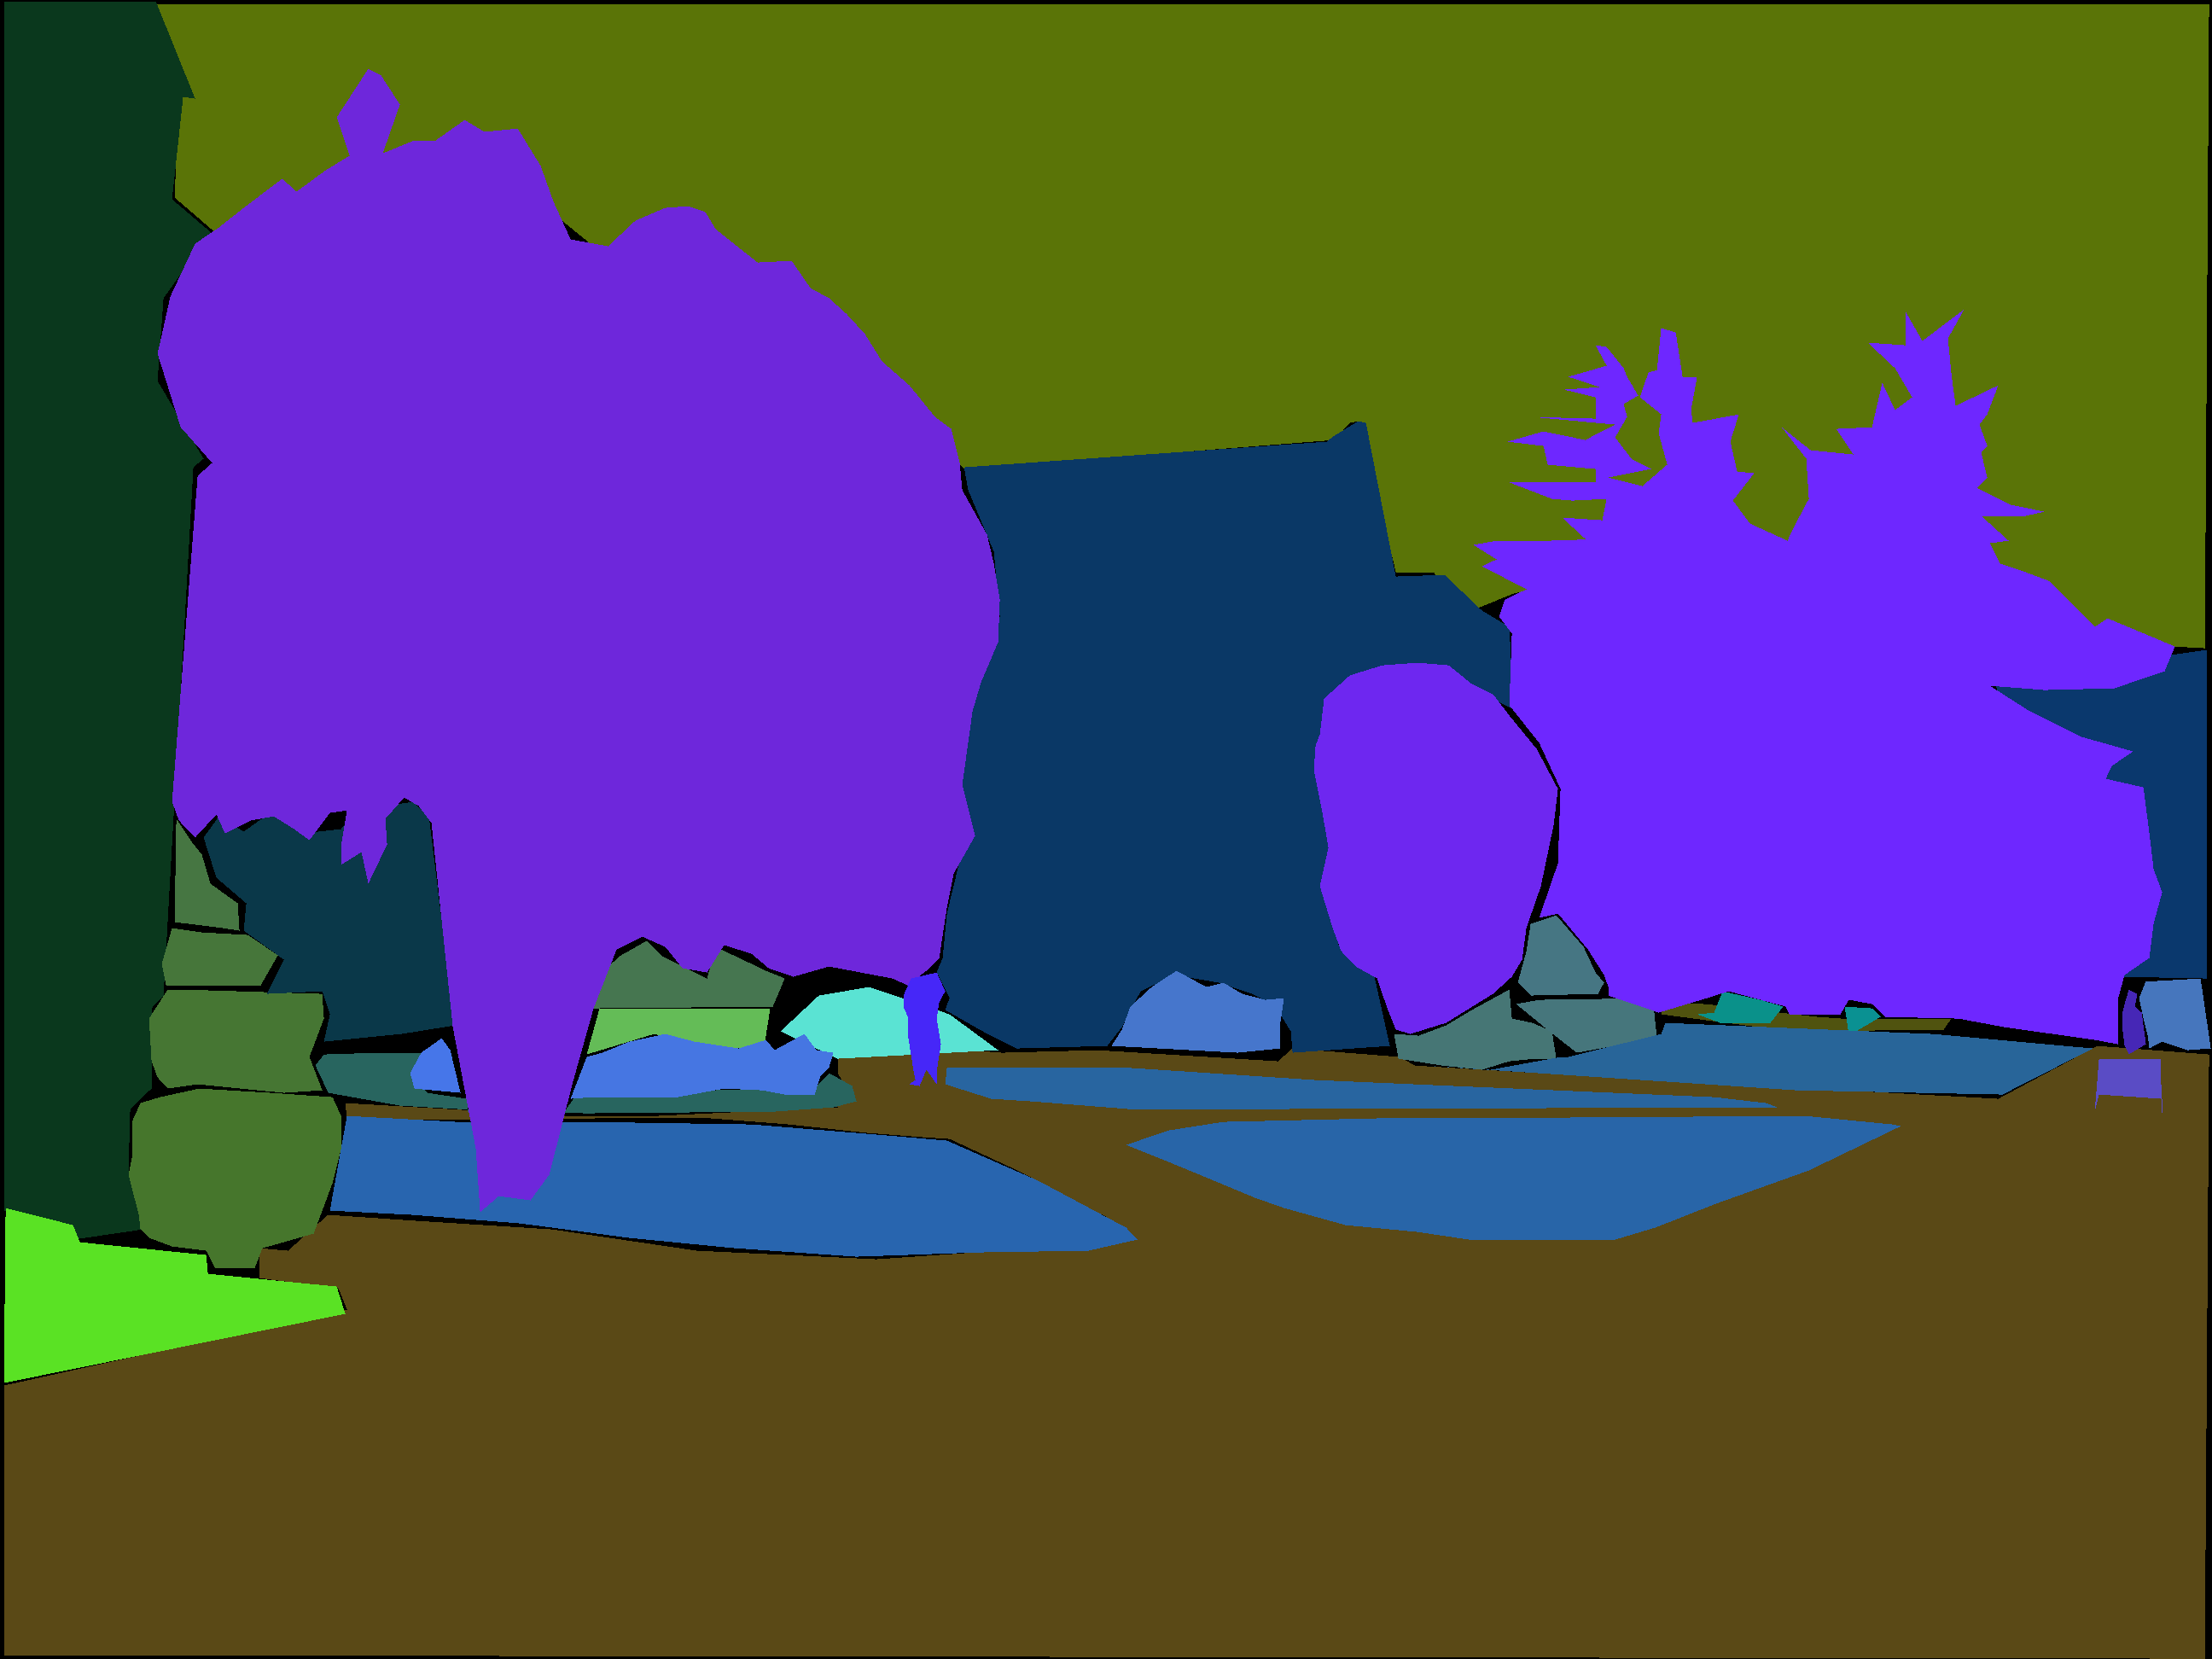
\includegraphics[width=9cm ,height=9cm ]{\output_image}};

    \draw[densely dashed]
    (image_1-nearnortheast) coordinate(a) -- (image_2-nearnorthwest)
    (image_1-nearsoutheast) coordinate(b) -- (image_2-nearsouthwest)
    (image_1-farsoutheast) coordinate(c) -- (image_2-farsouthwest)
    (image_1-farnortheast) coordinate(d) -- (image_2-farnorthwest);

    \draw [connection, ] (conv_68-west) -- node [fillwhite] {\midarrow}(soft_max-east);
    
    \pic[shift={(4, 0, 0)}] at (image_0.south east)
	{Box={
			name=spatial_mask,
			caption= ,
			zlabel=,
			fill=white,
			opacity=0.8,
			height=10.0,
			depth=10.0,
			width=0.5
		}
	};

    \draw [connection, pos=0.8]  (image_0.south)   |- node {\midarrow} (spatial_mask-west);

    \draw [connection, ] (conv_68-west) -- node [fillwhite] {\midarrow}(soft_max-east);

	\node[canvas is zy plane at x=0](grid_3) at (spatial_mask-east) {\drawcoloredgrid{2}{2}{0.66}{black}};
	
	\coordinate [shift={(-2, 2, 0)}] (dummy_mask) at (conv_68-far);

    \draw [connection, pos=0.8] (grid_3) -- node {} ++(8,0,0) -- node [fillwhite] {\midarrow} (dummy_mask) -- node {} ++(4, 0, 0) -- node {}(conv_68-far);

        \pic[shift={(15, 0, 0)}] at (image_2-south)
            {RightBandedBox={
                name=legend_1,
                fill=\ConvColor,
                bandfill=\ConvReluColor,
                height=5.0,
                depth=5.0,
                width={1.0}
            }
        };
        \node [shift={(0, -1.3, 0)}] at (legend_1-anchor) {\LARGE{Convolution layer}};

        \pic[shift={(5, 0, 0)}] at (legend_1-west)
        {Box={
                name=legend_2,
                fill=\PoolColor,
                height=5.0,
                depth=5.0,
                width={1}
            }
        };
        \node [shift={(0, -1.3, 0)}] at (legend_2-anchor) {\LARGE{Pooling layer}};

        \pic[shift={(5, 0, 0)}] at (legend_2-west)
        {Box={
                name=legend_3,
                fill=\UpsampleColor,
                height=5.0,
                depth=5.0,
                width={1}
            }
        };
        \node [shift={(0, -1.3, 0)}] at (legend_3-anchor) {\LARGE{Upsample layer}};

        \pic[shift={(5, 0, 0)}] at (legend_3-west)
        {Box={
                name=legend_4,
                fill=\SoftmaxColor,
                height=5.0,
                depth=5.0,
                width={1}
            }
        };
        \node [shift={(0, -1.3, 0)}] at (legend_4-anchor) {\LARGE{Softmax layer}};

        \pic[shift={(5, 0, 0)}] at (legend_4-west)
        {Box={
                name=legend_5,
                fill=white,
                height=5.0,
                depth=5.0,
                width={1}
            }
        };
        \node [shift={(0, -1.3, 0)}] at (legend_5-anchor) {\LARGE{Spatial mask}};

        \pic[shift={(5, 0, 0)}] at (legend_5-west)
        {Ball={
                name=legend_6,
                caption=,
                fill=\ConcColor,
                opacity=0.6,
                radius=2,
                logo=$\oplus$
            }
        };
        \node [shift={(0,-1.3,0)}] at (legend_6-anchor) {\LARGE{Concatenation}};

        \pic[shift={(5, 0, 0)}] at (legend_6-west)
        {Ball={
                name=legend_7,
                caption=,
                fill=\SumColor,
                opacity=0.6,
                radius=2,
                logo=$+$
            }
        };
        \node [shift={(0,-1.3,0)}] at (legend_7-anchor) {\LARGE{Summation}};     

        
        
   
    
        \end{tikzpicture}
        \end{document}
    